%
\label{Appendix}

\section{Working Example for Generating Counterfactuals}
\label{Appendix.WorkingExampleAAP}

In this section, we present a working example to illustrate counterfactual generation. 
Given the assumptions we make for a SCM $\mathcal{M}$ \eqref{eq:SCM} in Section~\ref{sec:CausalKnowledge} and the additional assumption of an additive noise model (ANM) in Section~\ref{sec:Experiments}, such procedure is straightforward.
Suppose we have the following SCM $\mathcal{M}$ and corresponding DAG $\mathcal{G}$:

%
\begin{minipage}{.45\linewidth}
\begin{figure}[H]
\centering
    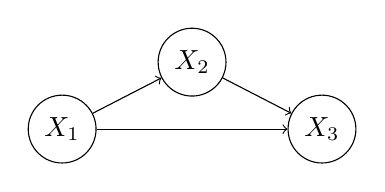
\begin{tikzpicture}
        \node (X1)  at (-1.65, 0) [circle, draw]{$X_1$};
        \node (X2) at (0, 0.85) [circle, draw]{$X_2$};
        \node (X3) at (1.65,0) [circle,draw]{$X_3$};
        % \node (Y)  at (1.75, 0) [circle, draw]{$\widehat{Y}$};
        \draw[->] (X1) to (X2) {};
        \draw[->] (X1) to (X3) {};
        % \draw[->] (X1) to (Y) {};
        \draw[->] (X2) to (X3) {};
        % \draw[->] (X2) to (Y) {};
    \end{tikzpicture}
\end{figure}
\end{minipage}
\begin{minipage}{.45\linewidth}
\begin{align*}
\mathcal{M} \, & 
\begin{cases}
    X_1 & \leftarrow U_1 \\
    X_2 & \leftarrow \alpha \cdot X_1  + U_2 \\
    X_3 & \leftarrow \beta_1 \cdot X_1 + \beta_2 \cdot X_2 + U_3
\end{cases}
\end{align*}
\end{minipage}
%

\medskip

\noindent
where $U_1, U_2, U_3$ represent the latent variables, $X_1, X_2, X_3$ the observed variables, and $\alpha, \beta_1, \beta_2$ the coefficient for the causal effect of, respectively, $X_1 \rightarrow X_2$,  $X_1 \rightarrow X_3$, and $X_2 \rightarrow X_3$. 
Suppose we want to generate the counterfactual for $X_3$, i.e., $X_3^{CF}$, had $X_1$ been equal to $x_1$. 
In the \textbf{abduction step}, we estimate $U_1$, $U_2$, and $U_3$ given the evidence, or what is observed, under the specified structural equations:
%
\begin{align*}
    \hat{U}_1 & = X_1 \\
    \hat{U}_2 & = X_2 - \alpha \cdot X_1 \\
    \hat{U}_3 & = X_3 - \beta_1 \cdot X_1 + \beta_2 \cdot X_2
\end{align*}
%
We generalize this step for \eqref{eq:SCM} as $U_j = X_j - f_j(X_{pa(j)})$ $\forall X_j \in X$. 
This step is an individual-level statement on the residual variation under SCM $\mathcal{M}$. 
It accounts for all that our assignment functions $f_j$, which are at the population level, cannot explain:~i.e., the \textit{error terms}. 
In the \textbf{action step}, we intervene $X_1$ and set all of its instances equal to $x_1$ via $do(X_1:=x_1)$ and obtain the intervened DAG $\mathcal{G}'$ and SCM $\mathcal{M}'$:

%
\begin{minipage}{.45\linewidth}
\begin{figure}[H]
\centering
    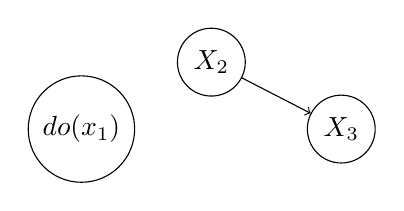
\begin{tikzpicture}
        \node (X1)  at (-1.65, 0) [circle, draw]{$do(x_1)$};
        \node (X2) at (0, 0.85) [circle, draw]{$X_2$};
        \node (X3) at (1.65,0) [circle,draw]{$X_3$};
        % \node (Y)  at (1.75, 0) [circle, draw]{$\widehat{Y}$};
        % \draw[->] (X1) to (X2) {};
        % \draw[->] (X1) to (X3) {};
        % \draw[->] (X1) to (Y) {};
        \draw[->] (X2) to (X3) {};
        % \draw[->] (X2) to (Y) {};
    \end{tikzpicture}
\end{figure}
\end{minipage}
\begin{minipage}{.45\linewidth}
\begin{align*}
\mathcal{M}' \, & 
\begin{cases}
    X_1 & = x_1 \\
    X_2 & \leftarrow \alpha \cdot x_1  + U_2 \\
    X_3 & \leftarrow \beta_1 \cdot x_1 + \beta_2 \cdot X_2 + U_3
\end{cases}
\end{align*}
\end{minipage}
%
\medskip

\noindent
where no edges come out from $X_1$ as it has been fixed to $x_1$. 
Finally, in the \textbf{prediction step}, we combine these two steps to calculate $X_3^{CF}$ under $\hat{U}$ and $\mathcal{M}'$:
%
\begin{align*}
    % X_1 &:= U_1 \\
    X_3^{CF} & \leftarrow \beta_1 \cdot x_1 + \beta_2 \cdot X_2 + \hat{U}_3 \\
             & \leftarrow \beta_1 \cdot x_1 + \beta_2 \cdot (\alpha \cdot x_1 + \hat{U}_2) + \hat{U}_3
\end{align*}
%
which is done for all instances in $X_3$. 
% This is what is done at a larger scale, for example, in \cite{Karimi2021_AlgoRecourse} and \cite{Pearl2016_CausalInference}, and also in this paper. 
The same three steps apply to $X_2$ and $X_1$.

We view the above approach as \textit{frequentist}, in particular, with regard to the abduction step.
% \footnote{This is not a formal distinction, but based on talks with other researchers. Such a distinction, to the best of our knowledge, remains an open question.} 
A more \textit{Bayesian} approach is what is done by \textcite{Kusner2017CF} in which they use a Monte Carlo Markov Chain (MCMC) to draw $\hat{U}$ by updating its prior distribution with the evidence $X$. 
In Section~\ref{sec:Experiments}, we used both approaches and found no difference in the results. 
In this work, we only present the results for the ``frequentist approach'' as it is less computationally expensive than running a MCMC. 

\section{Supplementary Material}
\label{Appendix.Supplements}

In this section, we present the supplementary material.

\subsection{Algorithms}

%
\begin{algorithm2e}[t]
\small %\scriptsize
    \caption{CST w/o $(\mathcal{D}, k, \tau, d)$}
    \label{alg:run_cfST}
	\SetKwInOut{Input}{Input}
	\SetKwInOut{Output}{Output}
	\Input{$\mathcal{D}$ - dataset, $k$ - neighborhood size, $\tau$ accepted deviation, $d$ distance function}
	\Output{$\mathcal{R}$ - set of pairs $(c, \Delta)$ of protected instance indexes and their $\Delta > \tau$}
	\BlankLine
	$\mathcal{D}_c=\{(x_i, a_i, \widehat{y}_i) \in \mathcal{D}: a_i=1\}$; \hfill\texttt{\scriptsize// control search space}\\
    $\mathcal{D}_t=\{(x_i, a_i, \widehat{y}_i) \in \mathcal{D}: a_i=0\}$\hfill\texttt{\scriptsize// test search space}\\
    $\mathcal{R} = \emptyset$\\
	\For{$(x_c, a_c, \widehat{y}_c) \in \mathcal{D}_c$}{
    $\text{\textit{k-ctr}} =
    \{ (x_i, a_i, \widehat{y}_i) \in \mathcal{D}_c: rank_{d}( x_c, x_i) \leq k \}$\hfill\texttt{\scriptsize// control group}\\
    $\text{\textit{k-tst}} = \{ (x_i, a_i, \widehat{y}_i) \in \mathcal{D}_t: rank_{d}( x^{CF}_c, x_i) \leq k \}$\hfill\texttt{\scriptsize// test group}\\
    $p_c = |\{ (x_i, a_i, \widehat{y}_i) \in \text{\textit{k-ctr}}: \hat{y}_i = 0 \}|/{k}$\hfill\texttt{\scriptsize// fraction of negative decisions for control}\\
    $p_t = |\{ (x_i, a_i, \widehat{y}_i) \in \text{\textit{k-tst}}: \hat{y}_i = 0 \}|/{k}$\hfill\texttt{\scriptsize// fraction of negative decisions for test}\\
    $\Delta = p_c - p_t$\hfill\texttt{\scriptsize// delta}\\
    \If{$\Delta > \tau$}{
    $\mathcal{R} = \mathcal{R} \cup \{(c, \Delta)\}$\hfill\texttt{\scriptsize// add pair to the result}\\
    }
	}
    \Return{$\mathcal{R}$}
\end{algorithm2e}
%

Algorithm~\ref{alg:run_cfST} reports the pseudo-code of the k-NN CST w/o algorithm. The pseudo-code is self-explanatory. 
After selecting the control and test search space (lines 1--2) as stated in Definition~\ref{def:SearchSpaces}, the algorithm iterates over the protected instances. For each of such instances, i.e., the complainant $c$, it builds (lines 5--6) the control and test groups as the $k$-nearest neighborhood instances relative to the distance $d$ for $x_c$ and for its counterfactual~$x^{CF}_c$ respectively, as stated in \eqref{eq:kctr} and \eqref{eq:ktst}. Then, the fractions $p_c$ and $p_t$ of negative decisions for the two groups are computed (lines 7--8) as stated in \eqref{eq:p1_and_p2}, as well as their difference $\Delta$ (line 9). If such a $\Delta$ is larger than the accepted deviation $\tau$, then the complainant $c$ and its $\Delta$ are added (lines 10--11) to the result $\mathcal{R}$.
%
The pseudo-code of k-NN CST w/ is a simple variant of Algorithm~\ref{alg:run_cfST}, which adds the search centers $x_c$ and $x^{CF}_c$ into the control and test groups, respectively, and divides by $k+1$ instead of $k$ at lines 7--8.

\subsection{Positive Discrimination}

Based on the discussion in Section~\ref{sec:CST_Disc}, we revisit Definitions \ref{def:IndDisc} and \ref{def:CIs} for testing individual positive discrimination under the k-NN CST. We still consider $\Delta p$ \eqref{eq:delta} and the converse of the one-sided CI $\eqref{eq:CIs}$. 

%
\begin{definition}[Positive Individual Discrimination]
\label{def:PostIndDisc}
    There is (potential) positive individual discrimination in favor of the complainant $c$ if $\Delta p < \tau$, meaning the negative decision outcomes rate for the control group is smaller than for the test group given some accepted deviation $\tau \in  [-1, 1]$.
\end{definition}
%

%
\begin{definition}[Confidence on the Positive Individual Discrimination Claim]
\label{def:PostCIs}
    A detected (potential) positive discrimination claim for the complainant $c$ by Definition~\ref{def:IndDisc}
    % by $\Delta p$ \eqref{eq:delta}  
    is statistically significant with significance level $\alpha$ if the CI $(- \infty, \Delta p + w_\alpha]$ excludes $\tau$.
\end{definition}
%

The concept of positive discrimination also applies to the case of multidimensional discrimination in Section~\ref{sec:CST.Multi}.
In that case, we would re-visit Definitions \ref{def:MultipleDisc} and \ref{def:IntersectionaleDisc} by looking at the opposite effect for $\Delta p$ across the protected attributes, be it each one of them or their intersection. 
We do not proceed with redefining these two definitions as we do not showcase them.
Again, especially for multidimensional discrimination, our focus is on discrimination \textit{against} protected groups.
Further, it is unclear what the legal scholarship views as positive multidimensional discrimination: from \textcite{Crenshaw1989_DemarginalizingTheIntersection} to \textcite{Xenidis2020_TunningEULaw}, the focus has been always on traditional discrimination.

\section{Additional Experiments}
\label{Appendix.AddExperiments}

In this section, we present additional experiments relative to the setup of Section~\ref{sec:Experiments}.

\subsection{Single Positive Discrimination}

For the same setup as in Section~\ref{sec:Experiments.SetUp} and the same data (factual and counterfactual) as in Section~\ref{sec:Experiments.IllustrativeExample}, we test for positive discrimination using Definitions \ref{def:PostIndDisc} and \ref{def:PostCIs}.
Regarding counterfactual fairness (CF), we define as positive CF discrimination when the factual has a positive decision outcome, $\hat{y}_c=1$ but its counterfactual a negative one, $\hat{y}_c^{CF}=0$.
Table~\ref{table:k-results_pos} summarizes the results for the protected attribute gender.

%
\begin{table}[t]
  \caption{Number (and \% females) of positive individual discrimination cases in Section~\ref{sec:Experiments.IllustrativeExample} based on gender. Marked by * are the statistically significant cases}
  \label{table:k-results_pos}
  \centering
  \begin{tabular}{clllll}
    \toprule
    Method & $k=15$ & $k=30$ & $k=50$ & $k=100$ & $k=250$\\
    \midrule
    CST w/o & 0 (0.0\%) & 0 (0.0\%) & 0 (0.0\%) & 0 (0.0\%)  & 0 (0.0\%) \\
     & 0* (0.0\%) & 0* (0.0\%) & 0* (0.0\%) & 0* (0.0\%)  & 0* (0.0\%) \\
     \midrule
    ST & 45 (2.6\%) & 50 (2.9\%) & 77 (4.5\%) & 118 (6.9\%) & 159 (9.3\%) \\
    & 41* (2.4\%) & 48* (2.8\%) & 55* (3.2\%) & 93* (5.4\%) & 120 (7.0\%) \\
    \midrule
    CST w/ & 0 (0.0\%) & 0 (0.0\%) & 0 (0.0\%) & 0 (0.0\%)  & 0 (0.0\%)\\
    & 0* (0.0\%) & 0* (0.0\%) & 0* (0.0\%) & 0* (0.0\%)  & 0* (0.0\%) \\
    \midrule
    CF & 0 (0.0\%) & 0 (0.0\%) & 0 (0.0\%) & 0 (0.0\%)  & 0 (0.0\%) \\
    & 0* (0.0\%) & 0* (0.0\%) & 0* (0.0\%) & 0* (0.0\%)  & 0* (0.0\%) \\
    \bottomrule
  \end{tabular}
\end{table}
%

Unlike all other single discrimination testing results in Section~\ref{sec:Experiments}, Table~\ref{table:k-results_pos} shows a ST that detects more cases than CST and a CST and CF that detect no cases at all. 
Both patterns hold when considering statistical significance.
These results are to be expected given how we generated the synthetic data for the loan application scenario. 
As described in Figure~\ref{fig:KarimiV2}, we introduced a negative systematic bias against female applicants in $\mathcal{D}$. 
This would explain why all the methods based on counterfactual generation---CF, CST w/, and CST w/o---detect zero cases: the generated male counterfactuals in $\mathcal{D}^{CF}$ can only improve over their female factual complainants in $\mathcal{D}$.
Hence, $\Delta p < \tau$ is very unlikely to occur when using CST or CF.
In other words, in a setting in which the protected individuals are always negatively affected in a systematic way, we should not expect to detect positive discrimination under methods that operationalize fairness given the difference.
Such results, for the purpose of this work, support our choice to consider only traditional discrimination as it is the most prevalent and important kind of discrimination when we suspect a negative systematic bias against the complainants. 

% Notably, 
Table~\ref{table:k-results_pos} raises questions on what kind of comparison is better suited for testing positive discrimination. 
The fact that ST, which uses an idealized comparison by implementing the CP manipulation, detects discrimination cases in a known biased setting for female applicants puts further into question the role of standard methods like it.
Is the idealized comparison suitable for positive discrimination or does \textcite{Kohler2018CausalEddie}'s criticism also apply to this setting?
Based on these preliminary results, we would argue that the tension between \textit{ceteris paribus} and \textit{mutatis mutandis} manipulations applies also to testing positive discrimination.
The stark difference between ST and CST in Table~\ref{table:k-results_pos} reinforces our view as, essentially, once we account for fairness given the difference in a known biased setting, it is difficult to argue that such a thing as positive discrimination occurs at all. 
Perhaps this is why this kind of discrimination is not discussed as much by legal scholars looking at indirect discrimination.
We plan to revisit these results in future work.

\subsection{Single Discrimination Testing}

We re-run Section~\ref{sec:Experiments.IllustrativeExample} and \ref{sec:Experiments.Real} for $\tau=0.05$, keeping all other parameters equal.
The results align with the ones we present in the main body. 
We focus on individual discrimination for all cases, not distinguishing between statistically and non-statistically significant cases.

Table~\ref{table:k-results_tau005} shows the same pattern between the CST versions relative to ST and CF as in Table~\ref{table:k-results}.
It illustrates the robustness of our framework. 
Two points we want to raise regarding Table~\ref{table:k-results_tau005}. 
First, CF, as expected, detects the same number of cases as it always looks for the strict equality between the factual and counterfactual quantities.
Second, under $\tau=0.05$, CST w/ and CST w/o align in the number of cases for larger $k$ sizes. This shows how influential $\tau$ can be for detecting discrimination, but also shows that either CST version can tackle the discrimination problem.
%
Tables \ref{table:k-results_RACE_tau005} and \ref{table:k-results_GENDER_tau005} show similar results as in, which are the $\tau=0.05$ counterparts of Tables \ref{table:k-results_RACE} and \ref{table:k-results_GENDER}. 
The results are expected given the setup. 
For both experiments the number of cases drops under $\tau=0.05$ as we have increased the difficulty of proving the individual discrimination claims.

%
\begin{table}[H]
  \caption{Number and (\% w.r.t. females) of cases based on $A$ in Figure~\ref{fig:KarimiV2}.}
  \label{table:k-results_tau005}
  \centering
  \begin{tabular}{lcccc}
    \toprule
    Method & $k=15$ & $k=30$ & $k=50$ & $k=100$ \\
    \midrule
    CST w/o & 288 (16.8\%) & 307 (17.9\%) & 331 (19.3\%) & 360 (21.0\%)  \\
    ST & 55 (3.2\%) & 60 (3.5\%) & 75 (4.4\%) & 79 (4.6\%) \\
    CST w/ & 420 (24.5\%) & 309 (18.1\%) & 334 (19.5\%) & 363 (21.2\%)  \\
    CF &  376 (22\%) &  376 (22\%) &  376 (22\%) & 376 (22\%)  \\
    \bottomrule
  \end{tabular}
\end{table}
%

%
\begin{table}[H]
  \caption{Number (and \% w.r.t.~non-whites) of cases based on $R$ using Figure~\ref{fig:LawSchool}.}
  \label{table:k-results_RACE_tau005}
  \centering
  \begin{tabular}{lccccc}
    \toprule
    Method & $k=15$ & $k=30$ & $k=50$ & $k=100$ \\
    \midrule
    CST w/o & 256 (7.30\%) & 301 (8.59\%) & 323 (9.21\%) & 376 (10.72\%)  \\
    ST & 33 (0.94\%) & 48 (1.37\%) & 57 (1.63\%) & 46 (1.31\%) \\
    CST w/ & 286 (8.16\%) & 301 (8.59\%) & 323 (9.21\%) & 376 (10.72\%)  \\
    CF &  231 (6.59\%) &  231 (6.59\%) &  231 (6.59\%) & 231 (6.59\%)  \\
    \bottomrule
  \end{tabular}
\end{table}
%
%
\begin{table}[H]
  \caption{Number (and \% w.r.t.~females) of cases based on $G$ Figure~\ref{fig:LawSchool}.}
  \label{table:k-results_GENDER_tau005}
  \centering
  \begin{tabular}{lcccc}
    \toprule
    Method & $k=15$ & $k=30$ & $k=50$ & $k=100$ \\
    \midrule
    CST w/o & 78 (0.82\%) & 105 (1.10\%) & 224 (2.35\%) & 231 (2.42\%)  \\
    ST & 77 (0.81\%) & 92 (0.96\%) & 181 (1.90\%) & 185 (1.94\%) \\
    CST w/ & 99 (1.04\%) & 105 (1.10\%) & 224 (2.35\%) & 231 (2.42\%)  \\
    CF &  56 (0.59\%) &  56 (0.59\%) &  56 (0.59\%) & 56 (0.59\%)  \\
    \bottomrule
  \end{tabular}
\end{table}
%

%
% EOS
%



% We present the relevant algorithms for the k-NN CST implementation (Section~\ref{sec:CST.AnImplementation}). The algorithm~\ref{alg:run_cfST} performs CST while algorithm~\ref{alg:get_topk} returns the indices of the top-$k$ tuples with respect to the search centers based on the distance function $d$. Notice that the main difference in algorithm~\ref{alg:run_cfST} when creating the neighborhoods is that the search centers are drawn from the factual dataset for the control group $\mathcal{D}$ and the counterfactual dataset $\mathcal{D}^{CF}$ for the test group. Further, notice that we use the same $c$ (i.e., index) for both as these two data-frames have the same structure by construction. 

% \newcommand\mycommfont[1]{\scriptsize\ttfamily\scriptsize{#1}}
% \SetCommentSty{mycommfont}

% \IncMargin{1.5em}
% \begin{algorithm2e}[h!]
% \small %\scriptsize
%     \caption{run\_CST}
%     \label{alg:run_cfST}
% 	\SetKwInOut{Input}{Input}
% 	\SetKwInOut{Output}{Output}
% 	\Input{$\mathcal{D}$, $\mathcal{D}^{CF}$, $k$}
% 	\Output{$[p_c - p_t]$}
% 	\BlankLine
% 	    $prot\_condition \leftarrow \mathcal{D}[:, \; prot\_attribute] == prot\_value$\\
% 	    $\mathcal{D}_c \leftarrow \mathcal{D}[prot\_condition]$\tcp*[f]{get protected (control) search space}\\
% 	    $\mathcal{D}_t \leftarrow \mathcal{D}[\neg \; prot\_condition]$\tcp*[f]{get non-protected (test) search space}\\
% 	    $prot\_idx \leftarrow \mathcal{D}_c.index.to\_list(\;)$\tcp*{get idx for all complainants}
% 	    $diff\_list = [ \; ]$ \\
% 	    \For{$c, \; row \in prot\_idx$}{
%         $res\_1 \leftarrow get\_top\_k(\mathcal{D}\; \; \; \; \; [c, \; :], \mathcal{D}_c, k)$\tcp*{idx of the top-k tuples for control group} 
%         $res\_2 \leftarrow get\_top\_k(\mathcal{D}^{CF}[c, \; :], \mathcal{D}_t, k)$\tcp*{idx of the top-k tuples for test group} 
%         $p_c \leftarrow sum(\mathcal{D}[res_1, \; target\_attribute]==negative\_outcome) \; / \; len(res\_1)$ \\
%         $p_t \leftarrow sum(\mathcal{D}[res_2, \; target\_attribute]==negative\_outcome) \; / \; len(res\_2)$ \\
%         $diff\_list[c] \leftarrow p_c - p_t$}
%     % \BlankLine
%     \Return{$diff\_list$}
%     % };\\ 
% \end{algorithm2e}

% \IncMargin{1.5em}
% \begin{algorithm2e}[h!]
% \small %\scriptsize
%     \caption{get\_top\_k}
%     \label{alg:get_topk}
% 	\SetKwInOut{Input}{Input}
% 	\SetKwInOut{Output}{Output}
% 	\Input{$t$, $t\_set$, $k$}
% 	\Output{$[indices]$}
% 	\BlankLine
%     % $(idx, dist) \leftarrow k\_NN(t, t\_set, k)$\tcp*{run k-NN algorithm}
%      $(idx, dist) \leftarrow k\_NN(t, t\_set, k + 1)$\tcp*{run k-NN algorithm with $k+1$}
%     \If{without search centers} {
%         $remove(t, idx, dist)$\tcp*{remove the center t from idx}
% %        \State $(idx, dist) \leftarrow k\_NN(t, t\_set, k + 1)$\tcp*{run k-NN algorithm with $k+1$}
%     }%\Else{
% %        \State $(idx, dist) \leftarrow k\_NN(t, t\_set, k)$\tcp*{run k-NN algorithm}
% %        \State $remove\_t(idx, dist)$\tcp*{remove the center t from idx}
% %    }
%     $idx' \leftarrow sort(idx, dist)$\tcp*{sort idx by the distance}
% %    \BlankLine
%     \Return{$idx'$}
%     % };\\ 
% \end{algorithm2e}


